%Nama Kelompok: Sistem_Operasi_Deadlock
%Kelas: D4 TI 1B
%Alit Fajar Kurniawan(1174057) 
%Muhammad Iqbal Panggabean(1174063)
%Muhammad Afra Faris(1174041)
%Khadijah Hasanah Puteri Harahap(1174044)

\section {DEADLOCK}

\subsection {Deadlock}
\subsubsection {Pengertian Deadlock}
	Pada kesempatan ini saya akan menjelaskan tentang definisi Deadlock, Deadlock ialah suatu keadaan yang dimana dua proses atau lebih, saling menunggu proses untuk dapat melepaskan sumber daya yang sedang dijalankan. Misalnya proses A yang memperlukan suatu sumber daya, tetapi sumber saya tersebut sedang digunkana oleh proses lain. Untuk lebih paham mengenai pengertian dari deadlock dan bagaimana cara mengatasinya, anda dapat membandingkannya dengan situasi yang satu ini. Pertama, Dalam kehidupan kita tentu membutuhkan suatu pekerjaan, dan untuk memperoleh suatu pekerjaan, anda harus memiliki pengalaman yang baik, untuk dapat memiliki pengalaman yang baik anda harus bekerja.

	\begin{figure}[ht]
	\centerline{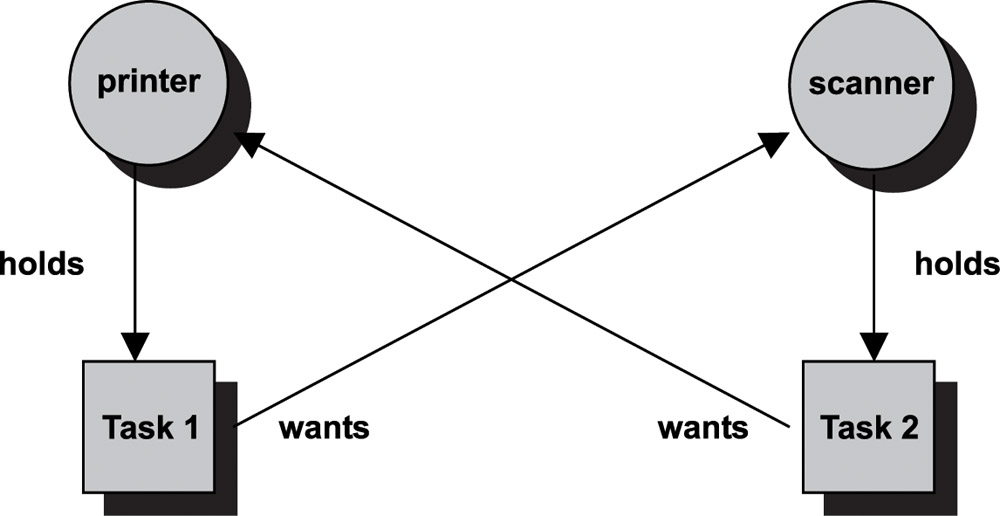
\includegraphics[width=1\textwidth]{figures/deadlock1.jpg}}
	\caption{Gambar Deadlock}
	\label{Gambar}
	\end{figure}
      
      Gambar \ref{Gambar_Deadlock} Contoh gambar pada saat terjadinya deadlock.

\subsection {Masalah Deadlock dan Metode Penanganan Deadlock}
\subsubsection {Masalah Deadlock}
	Deadlock merupakan dampak pengaruh dari sinkronisasi, yaitu dimana satu variabel yang digunakan oleh dua proses yang berbeda. Deadlock selalu tidak terlepas dari yang namanya sumber daya, karena hampir secara keseluruhan merupakan masalah mengenai sebuah sumber daya yang digunakan secara bersamaan. Sebuah Kelompok Proses yang diblok atau diblokir, dimana setiap proses memegang sebuah resource dan kemudian menunggu resource lain dari proses yang berada didalam proses yang sedang diBlok tersebut, biasanya dari semua proses-proses atau resource yang non preemptive.
	
\subsubsection {Metode Penanganan}
	Ada tiga Metode penanganan Deadlock:
	Yang Pertama yaitu, anda harus menggunakan satu protokol yang dapat membuat anda yakin bahwa sistem tersebut tidak akan pernah mengalami kejadian deadlock. Metode ini bisa disebut dengan Deadlock Prevention atau Avoidance.
	
	Yang Kedua, anda harus memberikan izin sistem untuk mengalami kejadian deadlock, namun setelah terjadinya deadlock anda harus dengan cepat segera untuk memperbaiki sistem yang mengalami deadlock tersebut. Metode ini biasanya disebut dengan Deadlock detection and recovery.
	
	Dan yang terakhir, anda hanya mengabaikan semua permasalahan yang terjadi secara bersamaan, dan kemudian menganggap bahwa deadlock tidak akan terjadi, metode ini digunakan dalam berbagai sistem operasi komputer, termasuk windows dan unix.

\begin{table}[H]
\begin{tabular}{|c|c|c|c|c|}
hline
Proses & Jumlah Sumber Daya Digenggam & Maksimum Sumber Daya Dibutuhkan\\
\hline
X   & 2 & 10\\
Y   & 1 & 3\\
Z   & 3 & 7\\
\hline
Tersedia 4
\hline
\end{tabular}
\end{table}

\subsection {Deadlock Detection}
\begin {enumerate}
\item
1. Pendeteksian secara Algoritma, yaitu dengan cara kita mengetahui jika terjadinya deadlock, deadlock terjadi jika suatu permintaan tidak dapat ditangani segera.
	
\item
2. Recovery atau Pemulihan, yaitu yang pertama menggagalkan semua proses deadlock, yang kedua mem backup semua proses yang deadlock dan kemudian silahkan melakukan restart di semua proses yang sedang terjadi, yang ketiga menggagalkan semua proses yang deadlock secara berurutan sehingga tidak akan terjadi lagi deadock, dan yang terakhir yaitu menggagalkan pengalokasian resource secara berurutan hingga tidak ada deadlock.

\end {enumerate}

\subsection {Beberapa hal yang terjadi ketika mendeteksi adanya deadlock}
\begin {enumerate}
\item
1. Permintaan sumber daya dikabulkan selama memungkinkan.
\item
2. Sistem operasi melakukan scanning apakah ada kondisi circular wait secara peiodik.
\item
3. Pemeriksaan dilakukan setiap ada sumber daya yang hendak digunakan.
\item
4. memeriksa dengan algoritma tertentu.
\end {enumerate}

\subsection {Beberapa jalan untuk kembali dari deadlock}
\begin {enumerate}
\item
1. Lewat Preemption, yaitu dengan jauhkan sumber daya dari pemakainya untuk sementara waktu, tujuannya untuk memberikannya pada proses lain. strategi dengan memberikannya kesempatan pada proses lain dengan tanpa diketahui oleh pemilik dari sumber daya itu dan tergantung juga dari sifat sumber daya itu sendiri.
\item
2. Lewat melacak kembali, setelah melakukan prosesn dari preemption tersebut maka secara otomatis proses utama yang diambil sumber dayanya akan stop dan tidak akan melanjutkan prosesnya, oleh karena itu dibutuhkan langkah untuk dapat kembali pada keadaan aman, tetapi untuk menentukan keadaan aman tersebut sangatlah susah.
\item
3. Mematikan proses yang menyebabkan deadlock, ini merupakan cara yang sangat umum digunakan yaitu dengan cara mematikan semua proses yang mengalami deadlock.
\item
4. Menghindari deadlock, pada sistem permintaan untuk sumberdaya biasanya hanya dilakukan sekali saja, sistem harus sudah dapat mengenali bahwa sistem itu aman atau tidak.
\end {enumerate}

\subsection {Reference}

@article{siahaan2015penyelarasan,
  title={Penyelarasan Pada Masalah Dining Philosophers Menggunakan Algoritma Lock \& Release},
  author={Siahaan, Andysah Putera Utama},
  journal={TECHSI-Jurnal Teknik Informatika},
  volume={7},
  number={1},
  year={2015}
}

@article{fauzi2013perangkat,
  title={PERANGKAT LUNAK VISUALISASI PERJALANAN KERETA API DENGAN MENGGUNAKAN PENDEKATAN SEMAPHORE, DEADLOCK SOLUTION DAN ALGORITMA DIJKSTRA},
  author={Fauzi, Esa},
  year={2013},
  publisher={Universitas Widyatama}
}

@book{silberschatz2014operating,
  title={Operating system concepts essentials},
  author={Silberschatz, Abraham and Galvin, Peter Baer and Gagne, Greg},
  year={2014},
  publisher={John Wiley \& Sons, Inc.}
}
